\section{From Observation to Action}
\label{sec:approach}
In this section, we describe how to derive search hints from performance data
to guide a search process.

\subsection{Exploration vs. Exploitation}

A search-based method navigates in the search space
to find the best cloud architectural configuration.
It is mostly concerned with
two questions:
``what are better choices?'' and
``what are more promising regions?''
The former ensures that a search will
eventually, find a near-optimal configuration
while
the latter determines how quickly it finds the solution
(also known as convergence speed).
An effective and efficient search method must answer
these two questions.

To this end, we actually need only to know ``what are better choices?''
At each step, a search-based method aims to find a cloud configuration
that is better than the current best.
A higher probability of \emph{guessing} the next step right
ensures that a search process sequentially finds a better choice.
A right next step also guides a search process
to move towards the right direction.
As long as the optimizer can move closer to the desired solution at each step,
it is more likely to guarantee it will find
near-optimal solutions.

To better determine the next step, a search process can learn
from the observations along the search path.
However, this method faces two challenges.
First, it requires collecting sufficient data to build strong belief.
\emph{CherryPick} is confronted by the cold-start issue
since it must first explore the search space---to identify the promising regions.
Second, an insufficient number of observations leads to
high bias in prediction---the method can wrongly believe that
a particular region (such as VM types or cluster sizes) is more promising
than the other, leading to a sub-optimal solution.

Instead of learning only from observations collected
while executing the target workload, a search process also can learn from
performance data of other workloads---which have been optimized in the past.
This addresses the issue of high bias because a larger number of
measurements (performance data) is available to create a prediction model that
generalizes a performance model better.
This also sidesteps the exploration problem because the search process
does not need to collect observations by running workloads
of the current search task.
The idea of reusing the data is often tricky
since the different combination of application and workload exhibit
very different behavior.
For example, the same application with different inputs can create
very different workload behavior
(such as the execution time and running cost)~\cite{Hsu2018Arrow}.
A performance model, which captures this complex behavior requires
more information about the search space than just
the architecture level information such as VM types and cluster sizes.


\subsection{Core Techniques}
To navigate the search space efficiently, \scout is built on
the following four ideas.


\subsubsection*{Pairwise comparison}
A search-based method determines the next configuration to evaluate.
That is, the method only needs to rank
the set of unevaluated cloud configurations.
Therefore, we can use \textit{Pairwise Comparison} modeling scheme~\cite{wauthier2013efficient}.
\emph{CherryPick} uses Gaussian process to build prediction model,
$f(x_i, K) = y_i$, where $x_i$ is the feature vector to represent
an architecture configuration and $K$ is the covariance kernel function.
With pairwise comparison, the learning task is
\begin{equation} \label{eq:1}
f(x_i, y_i, x_j) = y_j,
\end{equation}
where $x_i \in E$ and $x_j \in S-E$.
In words, it predicts the cost ($y_j$) of a configuration not yet
evaluated ($x_j$) given the cost ($y_i$) from the best configuration
yet found ($x_i$).
This modeling technique does not require to make an assumption ($K$) about
the search space (which is another hyper-parameter to tune),
and
naturally fits into SMBO in updating belief upon new observations.
For the same workload, switching
from a smaller VM type (\eg{\emph{large}}) to a larger one (\eg{\emph{2xlarge}})
may result in different performance on different VM families
(\eg{\emph{c4} and \emph{r4}}).
This performance relationship may change dramatically due to workload changes.
Regression-based modeling needs to fit the corresponding features accurately
for predicting performance~\cite{rasmussen2004gaussian,wettschereck1997review}.
Pairwise comparison helps capture performance transition
between architectural configurations.
Although there are $P(n,2)$ pairs (permutation),
where $n$ is the number of configurations,
in practice, we do not have to obtain full pairs for training this model.
This is because some pairs, \eg{(\emph{c4.large}, \emph{r4.large})}, show
significant performance differences in comparison with other pairs,
\eg{(\emph{m4.large}, \emph{r4.large})}.

\subsubsection*{Relative ordering}
Ranking architectural configurations does not need to predict
absolute performance (a harder problem).
Besides, ``a bad learner'' sometimes can still find a good solution~\cite{nair2017}. 
The idea of using an inaccurate model is useful
because the effort required to build an accurate model is much higher than
an inaccurate model.
%Hence, we do not need to predict performance directly rather
%the relative ordering or ranks.
%\ick[redundant with above?]
Based on this insight, we choose not to infer (inaccurate) performance measure
but rather to infer (accurate) relative ordering---
one configuration is better than another.
To support relative ordering, we modify the learning task from
\myequation{\ref{eq:1}} to
\begin{equation} \label{eq:2}
f(x_i, x_j) = \sigma({\frac{y_j}{y_i}})
\end{equation}
where $\sigma$ is a ranking function.
Binary ranking (\ie{better or worse}), for example, is the simplest form.
This transformation simplifies the learning task because
it does not predict absolute performance.
Furthermore, a coarse-grain ranking function better tolerates
performance variance in the cloud because
a small variance may still result in the same ranks.
%This technique trades search cost for search performance.
\myfigure{\ref{fig:reg_clas}} shows that the prediction accuracy of
relative ordering (using classification) is higher than
total ordering (using regression).
This experiment uses \emph{ExtraTrees}~\cite{geurts2006extremely} in
both the regression and classification task for fair comparison.
The increase in prediction accuracy greatly reduces search cost because
it is more likely to avoid wrong predictions (see Section~\ref{sec:why_better}).


\subsubsection*{Low-Level Insight}
Low-level performance metrics help identify
performance problems~\cite{Bodik2010, Novakovic2013} and
predict application and system performance~\cite{Hsu2016,Yadwadkar2017}.
Understanding resource bottlenecks helps choose the right cloud configuration and helps \scout ignore not so promising cloud configurations.
For example, in optimizing execution time, a memory bottleneck indicates
an instance with larger memory may improve resource efficiency,
thereby reducing execution time.
With low-level performance information, our learning task becomes
\begin{equation} \label{eq:3}
f(x_i, m_i, x_j) = \sigma({\frac{y_j}{y_i}})
\end{equation}
where $m_i$ represents the low-level performance vector.
This is similar to the process of
troubleshooting performance problems and
identifying resource bottleneck.
Instead of constructing rules manually,
this learning task can extract those rules implicitly.
When a workload runs inefficiently on one architectural configuration,
\scout observes abnormal or insufficient resource usage.
This observation is translated to prediction probability implicitly.
\scout ignores those configurations with low prediction probability.


\subsubsection*{Transfer learning}
The accuracy of a performance model depends on the number of data points
used to train the model.
In CAT, the data points are expensive to compute.
When building the performance models, it might be best to reference observations
from other optimization processes.
Researchers in transfer learning report that data
from other optimization processes can yield better models
than just using current data~\cite{pan2010survey,peters2015lace2}.
In this work, workloads share the same search space $S$ and therefore,
architectural features are the same.
Besides, \scout uses generic low-level metrics.
These enable transfer learning possible in \scout.
Although including workload information might improve search performance,
it prevents \scout from transferring knowledge
from historical optimization data.

\begin{figure}[t]
 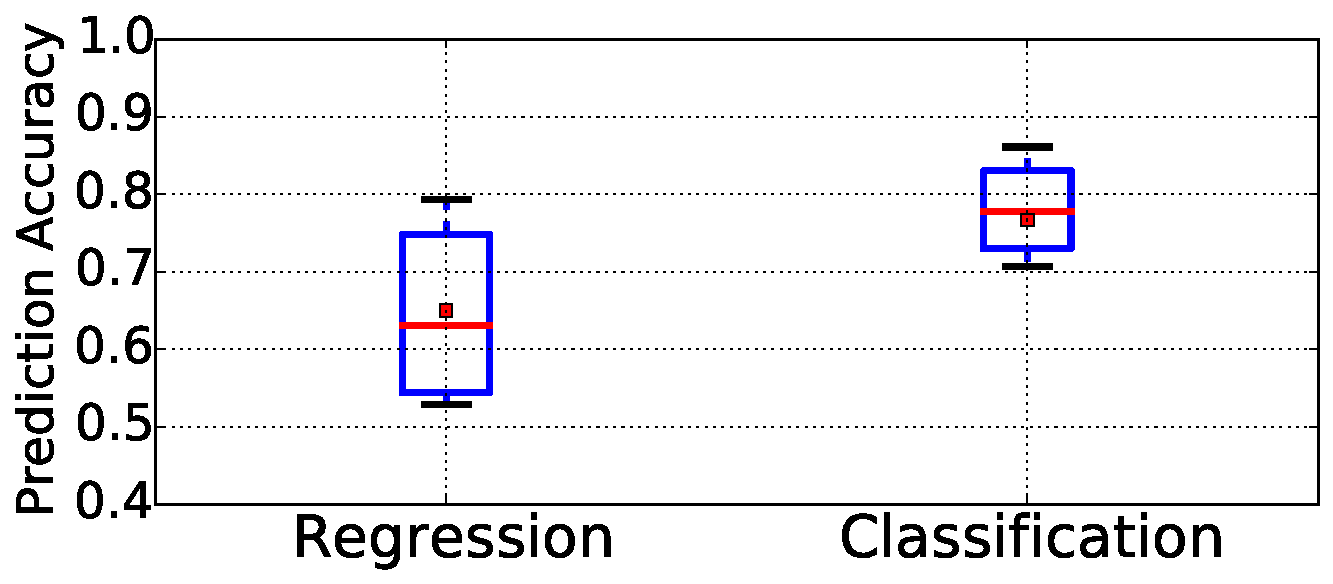
\includegraphics[width=.8\textwidth]{figures/multiple_prediction_accuracy.pdf}
 \centering
 \caption{\textbf{On the model selection of predicting the next step.}
 We evaluate the ability to distinguish a good and a bad configuration.
 In regression, we test rank preserving as prediction accuracy~\cite{nair2017}.}
 \label{fig:reg_clas}
\end{figure}


\subsection{Search Hints}
This section explains how to extract search hints using
probabilistic classification methods
~\cite{friedman2001elements,zadrozny2001obtaining,zadrozny2002transforming}.
A probabilistic classifier predicts probability distribution over
predicted classes.
In \myequation{\ref{eq:3}}, the learning task ranks the relative
performance measure of two architectural configurations.
We can map ranks to classes.
For example, the rank function $\sigma$ outputs \emph{class 1} if
$\frac{y_j}{y_i} < 1.1$. Otherwise, the output is \emph{class 0}.
A binary classifier is able to answer ``is $x_j$ better than $x_i$?''
A probabilistic classifier outputs higher probability for \emph{class 1} if
a specific workload performs better on $x_j$ than $x_i$.

We use an example to illustrate this process.
Consider a configuration space ($S=\{S_1, S_2, S_3, S_4\}$).
An CAT optimizer starts with $S_1$ and $y_1 = \phi(S_1) = 10$ (the current best).
Let us assume we have collected historical data for
training the probabilistic classifier.
The predicted probability distribution over ${S_1, S_2, S_3, S_4}$ 
is $[-, 0.8, 0.2, 0.2]$.
The probability vector $P_{i}$ represents
``how likely $S_j$ is a better choice than $S_i$.''
A higher value indicates $S_j$ is more likely
to perform better than $S_i$. 
In this example, $S_2$ is a better choice than the others.
When the actual performance measure is better $\phi(S_2) \leq \phi(S_1)$,
then CAT optimizer found a better solution than the current best.

The above example uses a binary classifier, and
\scout uses multiclass classification.
The intuition for using multiple classes is that some configurations
yield similar performance, and \scout should not consider little improvement.
For example, we can define the classes to be ``better,'' ``fair,'' and ``worse.''
\scout favors the configurations in the ``better'' class.
\scout uses a predefined discretization policy
(based on user-defined thresholds)  to convert probability to discrete classes.
%For example, $\frac{\phi(S_j)}{\phi(S_i)} \leq 0.8$ is considered as ``better.''
%\ick[do you mean i is better?]


\subsection{Search Strategy}

During the search process, a new observation
(running a workload on a selected cloud configuration)
provides the necessary information to determine
whether there exist better choices (see \myequation{\ref{eq:3}}).
The probability vector $P_{i}$ is derived
for each new observation $\phi(S_{i})$.
A search strategy determines the choice based on the probability predictions.
At each step, the search process selects the configuration $S_j$ with
the maximum probability in $P_{i}$.

This search strategy is similar to depth-first search.
While \emph{CherryPick} requires balancing exploration and exploitation,
\scout tends to exploit---because it uses historical data.
When the prediction model can generate quality predictions,
this search strategy leads to quick convergence speed
(the selected configuration improves over the current best).
Therefore, the search process has low search cost to find near-optimal
configurations. 

A search process should stop when it no longer can find a better configuration. This is controlled by a predefined parameter called  \textit{probability threshold} ($\alpha$) and acts as a stopping criterion.
When the predicted probability $P_{ij}$ is lower than $\alpha$ for all $S_j$,
the search process is not confident that it would find better configurations in the next step.
A search should also stop if it fails to find better solutions due to an inaccurate performance model. This is controlled by another parameter called \textit{ misprediction tolerance} ($\beta$) to avoid excessive search cost.

\subsection{Putting It All Together}
We have shown that the core element of a search based method is to determine
the next best step.
For obtaining hints to guide a search process,
we propose using the probabilistic classification technique
to predict improvement probability.
That is similar to Expected Improvement (EI) in \emph{CherryPick}.
We choose pairwise comparison and relative ordering
to deliver high prediction accuracy and to naturally into the search process.
\scout leverages low-level performance information and
extracts rules (based on resource utilization) implicitly.
This improves a search process because certain types of cloud configurations
can be avoided (as we will show in Section~\ref{sec:evaluation}).
Last, we choose a search strategy that merely picks the configuration
that is most likely to be better than the current best.
This strategy increases convergence speed---has low search cost.
